% !TeX TXS-program:compile = txs:///pdflatex/[--shell-escape]
\documentclass[letterpaper,12pt]{book}
\usepackage[margin=1in]{geometry}
\usepackage[utf8]{inputenc}
\usepackage[T1]{fontenc}
\usepackage{lmodern}
\usepackage{amsmath,amssymb}
\usepackage{siunitx}
\usepackage{graphicx}
\usepackage{pdfpages}
\usepackage{tikz}
\usetikzlibrary{
    arrows.meta,
    positioning,
    calc,
    fit,
    backgrounds,
    shapes.misc
}
\usetikzlibrary{arrows.meta,calc,positioning,shapes.geometric}
\usepackage{enumitem}
\usepackage{float}
\usepackage{booktabs}
\usepackage{longtable}
\usepackage{array}
\usepackage{tabularx}
\usepackage{pgfplotstable}
\usepackage{listings}
\usepackage{fancyhdr}
\usepackage{url}
\usepackage[hidelinks]{hyperref}
\usepackage{xcolor}
\usepackage{rotating}
\usepackage{adjustbox}

\setlength{\parindent}{0pt}
\setlength{\parskip}{0.5em}
\raggedbottom
\setlength{\headheight}{15pt}
\setcounter{secnumdepth}{3}
\setcounter{tocdepth}{2}
\pdfminorversion=7
\sisetup{detect-all}

\newcommand{\manualdate}{September 15, 2026}
\newcommand{\manualrev}{Rev. ET450-W1}
\newcommand{\appref}[1]{\hyperref[#1]{Appendix~\ref*{#1}}}

\fancyhf{}
\fancyhead[LE,RO]{\thepage}
\fancyfoot[L]{\manualdate}
\fancyfoot[C]{\manualrev}
\renewcommand{\headrulewidth}{0pt}
\renewcommand{\footrulewidth}{0.4pt}
\fancypagestyle{plain}{
    \fancyhf{}
    \fancyhead[LE,RO]{\thepage}
    \fancyfoot[L]{\manualdate}
    \fancyfoot[C]{\manualrev}
    \renewcommand{\headrulewidth}{0pt}
    \renewcommand{\footrulewidth}{0.4pt}
}

\author{Michael Capotosto}
\title{Multi-Rail Isolated Power Supply Monitoring System\\[0.5em]
    \large Capstone Design Documentation}
\date{\manualdate\\[1em]\small \manualrev}

\begin{document}
    \frontmatter
    \maketitle
    \tableofcontents
%    \listoffigures
%    \listoftables

    \mainmatter
    \pagestyle{fancy}

    % !TeX root = ../main.tex

\chapter{Introduction}
\label{chap:introduction}

\section{Project Overview}

The Multi-Rail Isolated Power Supply Monitoring System is a hardware and
software system developed to provide centralized monitoring of multiple
electrically isolated power-supply rails. The system measures both output
voltage and load current, provides configurable alarm
limits, displays operating status and measurement data via a local display or ethernet for integration with an EPICS-based control system.

The completed system monitors six independent power-supply rails:

\begin{itemize}
    \item +5VA
    \item +5VB
    \item +5V
    \item -5V
    \item +15V
    \item -15V
\end{itemize}

Because the monitored supplies may be electrically isolated from one another,
the monitoring system must preserve that isolation while still allowing all six
channels to communicate with a common controller. Each supply rail therefore
uses an independent voltage/current monitoring channel and an isolated digital
communication path.

The primary controller is an Arduino GIGA R1 WiFi. The controller acquires
measurement data from the individual monitor channels, converts the data to
engineering units, applies the appropriate rail polarity, evaluates configured
alarm limits, and presents the resulting information on a GIGA Display Shield.
An Ethernet interface provides network communication between the embedded
controller and an EPICS Input/Output Controller (IOC). The EPICS IOC then makes
the measurements, alarms, and system status available to a CS-Studio Phoebus
operator interface.


\section{Project Motivation}

Power-supply systems containing multiple isolated voltage rails present a
monitoring challenge because each circuit associated with one supply
can't share a direct electrical reference with another supply.
Connecting conventional measurement or communication circuits across these
references can break isolation between the rails.

A centralized monitor is desirable because it allows the user to observe all supply voltages and currents from a single interface,
identify abnormal operating conditions, detect communication or sensor faults,
and integrate the power-supply status into a larger control system.

The design developed for this project addresses these requirements by
performing voltage and high-side current measurement locally on each monitored
rail and transferring the resulting information across electrically isolated
digital interfaces. The controller receives measurement data from all
six rails without requiring their power references to be directly connected
together.


\section{System Architecture}

The monitoring system is divided into three primary functional areas:
the power-supply monitoring hardware, the microcontroller, and the
supervisory control interface.

The power supply monitoring hardware contains the current-sense resistors,
LTC2945 PMICs, and digital isolation circuitry. Each LTC2945 measures the supply
voltage and the differential voltage developed across a high-side current-sense
resistor. The resulting digital measurement information is sent over the I\textsuperscript{2}C bus while maintaining the required electrical isolation.

The Arduino GIGA R1 WiFi provides the mcu processing functions. Its
firmware initializes the monitoring channels, acquires voltage and current
measurements, detects communication errors, converts raw measurements to
engineering units, applies channel-specific polarity and scaling, evaluates
alarm limits, and updates the local display. Configuration information,
including network parameters and alarm limits, is retained in persistent
storage so that required settings can survive a controller reset or power
cycle.

Network communication is provided through an Ethernet interface using the PSC
protocol. The EPICS IOC communicates with the embedded controller using
PSCDriver and converts the transmitted values into EPICS process variables.
CS-Studio Phoebus provides the remote operator interface for viewing
measurements, alarm conditions, connection status, and system state.


\section{Design Objectives}

The major design objectives for the Multi-Rail Isolated Power Supply Monitoring
System are to:

\begin{enumerate}
    \item Measure the voltage of six independent power-supply rails.

    \item Measure the load current of each rail using high-side current sensing.

    \item Preserve electrical isolation between independently referenced
    power-supply rails and the common controller.

    \item Convert acquired data into meaningful engineering units and correctly
    represent both positive and negative voltage rails.

    \item Detect I\textsuperscript{2}C communication failures and prevent invalid
    sensor data from being presented as valid measurements.

    \item Compare voltage and current measurements against configurable upper and
    lower alarm limits.

    \item Provide a local graphical display of voltage, current, alarm status,
    communication status, and network state.

    \item Retain configuration and alarm settings through controller resets and
    power cycles.

    \item Provide Ethernet communication for remote monitoring and configuration.

    \item Integrate the monitoring system with an EPICS IOC and CS-Studio Phoebus
    operator interface.

    \item Maintain the hardware, firmware, and control-system software under
    revision control so that changes made during design, implementation, and
    testing remain traceable.
\end{enumerate}


\section{Project Scope}

The scope of the project includes the design and implementation of the sensor
interface hardware, Arduino GIGA controller hardware, embedded firmware,
Ethernet communication interface, EPICS IOC, and operator-interface software.
The hardware portion includes the six voltage/current monitoring channels,
current-sense resistors, digital isolation circuitry, controller interface,
Ethernet circuitry, and supporting power-supply circuitry.

The software portion includes the embedded acquisition and alarm-processing
firmware, persistent configuration storage, local display interface, PSC
network communication, EPICS IOC configuration and database records, and the
CS-Studio Phoebus operator interface.

Design files and software associated with the project are maintained in the
project Git repository:

\begin{center}
    \url{https://github.com/capotosto/PS_Monitor}
\end{center}

The repository provides revision control for the hardware design, firmware,
EPICS IOC files, documentation, and other project artifacts generated during
development.


\section{Report Organization}

This report documents the development of the monitoring system from preliminary
design through implementation and testing. The preliminary-design chapter
defines the major functional blocks, presents the system architecture,
documents supporting engineering calculations, includes the hardware
schematics and bills of materials, and describes the primary firmware and
control-system software flows.

Subsequent chapters document prototyping and development activities, the EPICS
IOC implementation, and the CS-Studio Phoebus operator interface. Supporting
project-management and design documents developed during the earlier phases of
the capstone project are retained as part of the overall project documentation
and provide traceability between the original requirements, design decisions,
implementation, and final system.
    % !TeX root = ../main.tex
\chapter{Preliminary Design (Week 1 Assignment)}
\label{chap:preliminary-design}

\section{Purpose and Scope}
This chapter documents the preliminary hardware and software design of the
Multi-Rail Isolated Power Supply Monitoring System. The design monitors six
power-supply rails, measures rail voltage and load current, preserves electrical
isolation between floating supplies and the controller, evaluates measurements
against user-configurable alarm limits, presents local status on the controller
display, and publishes measurements and status to an EPICS control-system
interface.

This preliminary design is intended to establish the major analog and digital
functional blocks, document supporting engineering calculations, define the
hardware schematic baseline, and provide software flowcharts detailed enough to
support implementation. Simulation and additional verification results can be
added in the subsequent design phase.

\section{Major Functional Blocks}
\label{sec:functional-blocks}
The major system functions are summarized below.

\begin{enumerate}
    \item \textbf{Power-Supply Interface:} Connect to the six monitored rails and
    route each rail through the associated voltage/current monitoring channel.
    \item \textbf{Current Measurement:} Convert load current to a differential
    voltage across a precision shunt resistor and digitize it with the
    LTC2945.
    \item \textbf{Voltage Measurement:} Measure the monitored rail voltage using
    the LTC2945 supply-voltage ADC channel.
    \item \textbf{Electrical Isolation:} Maintain galvanic isolation between each
    floating monitored supply and the common controller-side I\textsuperscript{2}C bus.
    \item \textbf{Digital Acquisition:} Poll each monitor, identify communication
    faults, apply channel-specific sign/scaling information, and calculate
    engineering-unit values.
    \item \textbf{Alarm Processing:} Compare voltage and current values against
    configured upper and lower limits and generate channel alarm states.
    \item \textbf{Local User Interface:} Present all rail measurements, alarms,
    network state, and communication status on the Arduino GIGA Display.
    \item \textbf{Network/EPICS Interface:} Publish measurements, alarm limits,
    alarm state, and connection status over Ethernet for the EPICS IOC and
    Phoebus interface.
\end{enumerate}

\subsection{Functional Block Diagram}

% The complete diagram and its caption are rotated together, but the enclosing
% figure uses [H], so LaTeX keeps the figure at this location in the source.
% Requires \usepackage{graphicx}, \usepackage{tikz}, and \usepackage{float}.
\begin{figure}[H]
    \centering

    % Center the rotated diagram/caption assembly on the portrait page.
    \makebox[\textwidth][c]{%
        \rotatebox{90}{%
            \begin{minipage}{0.9\textheight}
                \centering

                % Scale the complete TikZ drawing as one object while preserving
                % its aspect ratio.
                \resizebox{0.78\textheight}{!}{%
                    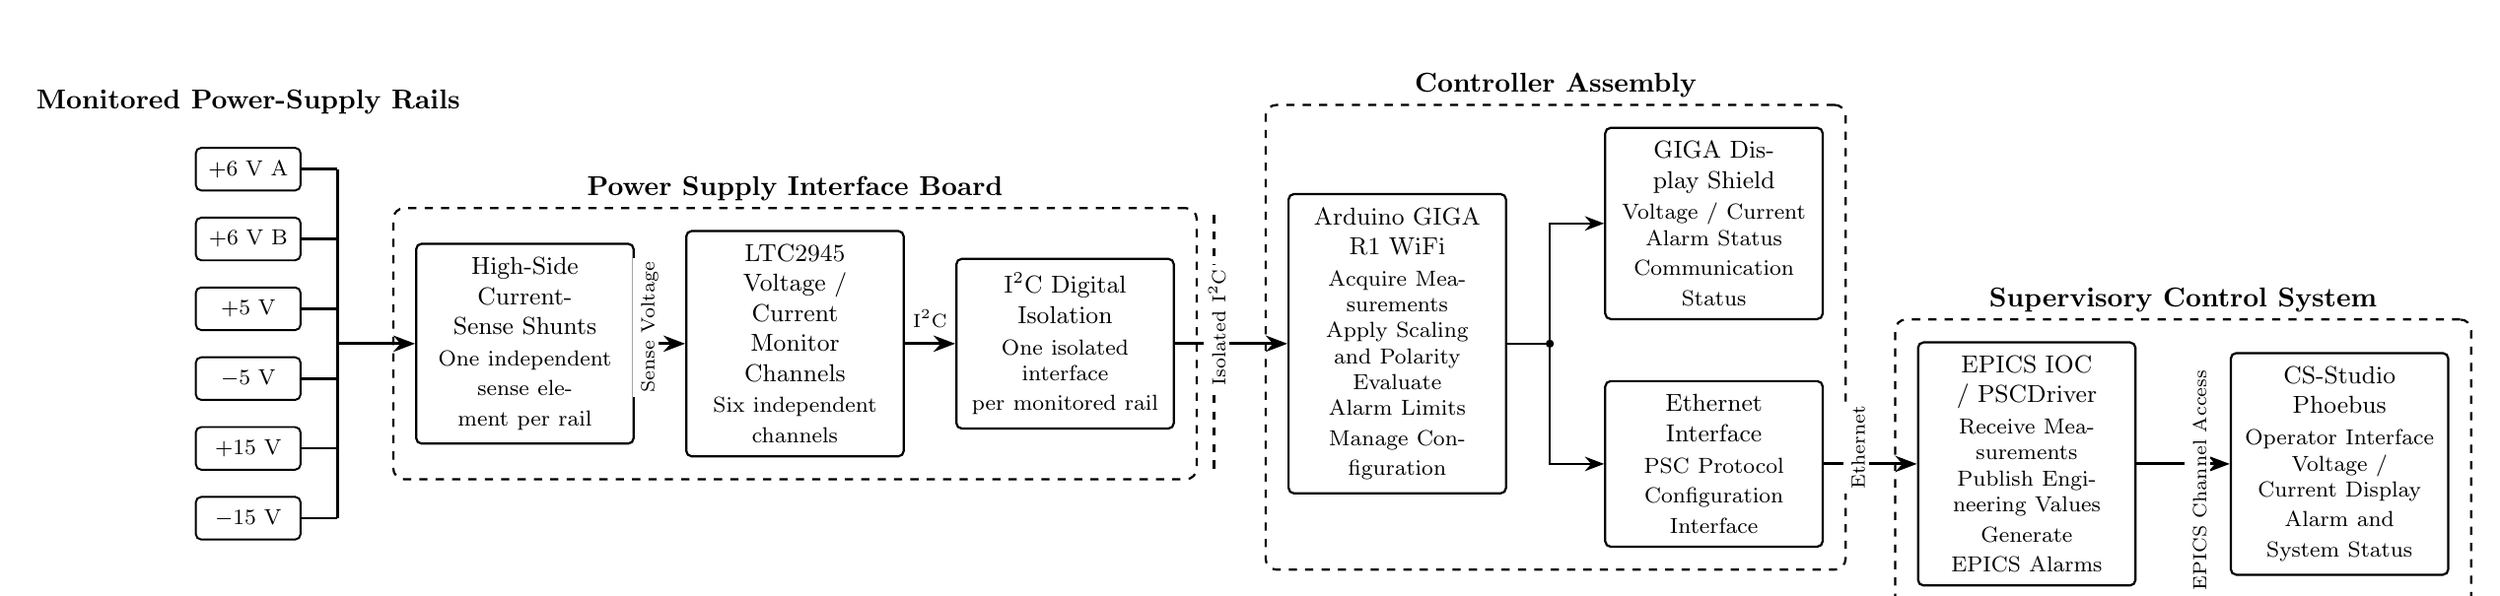
\begin{tikzpicture}[
                        >=Stealth,
                        font=\small,
                        block/.style={
                            draw,
                            rectangle,
                            rounded corners=2pt,
                            align=center,
                            minimum height=1.25cm,
                            minimum width=2.75cm,
                            text width=2.45cm,
                            inner sep=5pt,
                            line width=0.8pt
                        },
                        rail/.style={
                            draw,
                            rectangle,
                            rounded corners=2pt,
                            align=center,
                            minimum height=0.55cm,
                            minimum width=1.35cm,
                            font=\footnotesize,
                            line width=0.7pt
                        },
                        group/.style={
                            draw,
                            dashed,
                            rounded corners=4pt,
                            inner sep=8pt,
                            line width=0.8pt
                        },
                        signal/.style={
                            ->,
                            line width=0.9pt
                        },
                        line/.style={
                            line width=0.9pt
                        },
                        bus/.style={
                            line width=1.1pt
                        },
                        busarrow/.style={
                            ->,
                            line width=1.1pt
                        },
                        siglabel/.style={
                            font=\scriptsize,
                            fill=white,
                            inner sep=1.5pt,
                            text depth=0pt,
                            text height=1.5ex,
                            align=center
                        }
                        ]

                        % ============================================================
                        % MONITORED POWER RAILS
                        % ============================================================

                        \node[rail] (p6a) at (0, 2.25) {+6 V A};
                        \node[rail] (p6b) at (0, 1.35) {+6 V B};
                        \node[rail] (p5)  at (0, 0.45) {+5 V};
                        \node[rail] (m5)  at (0,-0.45) {$-5$ V};
                        \node[rail] (p15) at (0,-1.35) {+15 V};
                        \node[rail] (m15) at (0,-2.25) {$-15$ V};

                        \node[
                        above=0.30cm of p6a,
                        font=\bfseries
                        ] {Monitored Power-Supply Rails};


                        % ============================================================
                        % RAIL COLLECTION BUS
                        % ============================================================

                        \coordinate (railBusTop)    at (1.15, 2.25);
                        \coordinate (railBusBottom) at (1.15,-2.25);
                        \coordinate (railBusMid)    at (1.15, 0);

                        \draw[bus] (railBusTop) -- (railBusBottom);

                        % Individual rail connections -- no overlapping arrowheads.
                        \foreach \railname/\y in {
                            p6a/2.25,
                            p6b/1.35,
                            p5/0.45,
                            m5/-0.45,
                            p15/-1.35,
                            m15/-2.25
                        }{
                            \draw[line] (\railname.east) -- (1.15,\y);
                        }


                        % ============================================================
                        % POWER-SUPPLY INTERFACE BOARD
                        % ============================================================

                        \node[
                        block,
                        anchor=west
                        ] (shunts) at (2.15,0)
                        {
                            High-Side\\
                            Current-Sense Shunts\\[2pt]
                            \footnotesize
                            One independent\\
                            sense element per rail
                        };

                        \node[
                        block,
                        right=0.65cm of shunts
                        ] (ltc)
                        {
                            LTC2945\\
                            Voltage / Current\\
                            Monitor Channels\\[2pt]
                            \footnotesize
                            Six independent\\
                            channels
                        };

                        \node[
                        block,
                        right=0.65cm of ltc
                        ] (iso)
                        {
                            I\textsuperscript{2}C Digital\\
                            Isolation\\[2pt]
                            \footnotesize
                            One isolated interface\\
                            per monitored rail
                        };

                        % One clean arrow from the six-rail collection bus.
                        \draw[busarrow]
                        (railBusMid)
                        --
                        (shunts.west);

                        % Shunt -> LTC.  Vertical text avoids overlap with the boxes.
                        \draw[busarrow]
                        (shunts.east)
                        --
                        node[
                        siglabel,
                        midway,
                        rotate=90,
                        above=6pt
                        ]
                        {Sense Voltage}
                        (ltc.west);

                        % LTC -> isolation.  This short label remains horizontal.
                        \draw[busarrow]
                        (ltc.east)
                        --
                        node[
                        siglabel,
                        midway,
                        above=4pt
                        ]
                        {I\textsuperscript{2}C}
                        (iso.west);


                        % ============================================================
                        % POWER-SUPPLY INTERFACE GROUP
                        % ============================================================

                        \begin{scope}[on background layer]
                            \node[
                            group,
                            fit=(shunts)(ltc)(iso)
                            ] (interfaceGroup) {};
                        \end{scope}

                        \node[
                        font=\bfseries,
                        fill=white,
                        inner sep=2pt,
                        anchor=south
                        ]
                        at (interfaceGroup.north)
                        {Power Supply Interface Board};


                        % ============================================================
                        % ISOLATION BARRIER
                        % ============================================================

                        \coordinate (barrierTop)
                        at ($(iso.north east)+(0.50,0.55)$);

                        \coordinate (barrierBottom)
                        at ($(iso.south east)+(0.50,-0.55)$);

                        % Keep only the dashed isolation-barrier line; no text label.
                        \draw[
                        dashed,
                        line width=1.1pt
                        ]
                        (barrierTop) -- (barrierBottom);


                        % ============================================================
                        % ARDUINO GIGA
                        % ============================================================

                        \node[
                        block,
                        right=1.45cm of iso
                        ] (giga)
                        {
                            Arduino GIGA R1 WiFi\\[2pt]
                            \footnotesize
                            Acquire Measurements\\
                            Apply Scaling and Polarity\\
                            Evaluate Alarm Limits\\
                            Manage Configuration
                        };

                        % Isolation -> Arduino.  Vertical text prevents overlap.
                        \draw[busarrow]
                        (iso.east)
                        --
                        node[
                        siglabel,
                        midway,
                        rotate=90,
                        above=6pt
                        ]
                        {Isolated I\textsuperscript{2}C}
                        (giga.west);


                        % ============================================================
                        % DISPLAY AND ETHERNET
                        % ============================================================

                        \node[
                        block,
                        right=1.25cm of giga,
                        yshift=1.55cm
                        ] (display)
                        {
                            GIGA Display Shield\\[2pt]
                            \footnotesize
                            Voltage / Current\\
                            Alarm Status\\
                            Communication Status
                        };

                        \node[
                        block,
                        right=1.25cm of giga,
                        yshift=-1.55cm
                        ] (ethernet)
                        {
                            Ethernet Interface\\[2pt]
                            \footnotesize
                            PSC Protocol\\
                            Configuration Interface
                        };

                        % Branch after the Arduino so the two output arrows do not
                        % overlap each other.
                        \coordinate (controllerBranch)
                        at ($(giga.east)+(0.55,0)$);

                        \draw[line]
                        (giga.east)
                        --
                        (controllerBranch);

                        \draw[signal]
                        (controllerBranch)
                        |-
                        (display.west);

                        \draw[signal]
                        (controllerBranch)
                        |-
                        (ethernet.west);

                        \fill (controllerBranch) circle (1.5pt);


                        % ============================================================
                        % CONTROLLER GROUP
                        % ============================================================

                        \begin{scope}[on background layer]
                            \node[
                            group,
                            fit=(giga)(display)(ethernet)
                            ] (controllerGroup) {};
                        \end{scope}

                        \node[
                        font=\bfseries,
                        fill=white,
                        inner sep=2pt,
                        anchor=south
                        ]
                        at (controllerGroup.north)
                        {Controller Assembly};


                        % ============================================================
                        % EPICS IOC
                        % ============================================================

                        \node[
                        block,
                        right=1.20cm of ethernet
                        ] (ioc)
                        {
                            EPICS IOC / PSCDriver\\[2pt]
                            \footnotesize
                            Receive Measurements\\
                            Publish Engineering Values\\
                            Generate EPICS Alarms
                        };

                        % Ethernet -> IOC.  Vertical text prevents overlap.
                        \draw[busarrow]
                        (ethernet.east)
                        --
                        node[
                        siglabel,
                        midway,
                        rotate=90,
                        above=6pt
                        ]
                        {Ethernet}
                        (ioc.west);


                        % ============================================================
                        % PHOEBUS
                        % ============================================================

                        \node[
                        block,
                        right=1.20cm of ioc
                        ] (phoebus)
                        {
                            CS-Studio Phoebus\\[2pt]
                            \footnotesize
                            Operator Interface\\
                            Voltage / Current Display\\
                            Alarm and System Status
                        };

                        % IOC -> Phoebus.  Vertical text prevents overlap.
                        \draw[busarrow]
                        (ioc.east)
                        --
                        node[
                        siglabel,
                        midway,
                        rotate=90,
                        below=6pt
                        ]
                        {EPICS Channel Access}
                        (phoebus.west);


                        % ============================================================
                        % SUPERVISORY GROUP
                        % ============================================================

                        \begin{scope}[on background layer]
                            \node[
                            group,
                            fit=(ioc)(phoebus)
                            ] (supervisoryGroup) {};
                        \end{scope}

                        \node[
                        font=\bfseries,
                        fill=white,
                        inner sep=2pt,
                        anchor=south
                        ]
                        at (supervisoryGroup.north)
                        {Supervisory Control System};

                    \end{tikzpicture}%
                }

                \vspace{0.25cm}

                % Because the caption is inside the rotated minipage, the figure
                % number, caption text, and diagram rotate together.
                \caption{
                    Preliminary functional block diagram of the multi-rail isolated
                    power supply monitoring system. Six independent power-supply rails
                    are measured using high-side current sensing and LTC2945 voltage/current
                    monitoring channels. Digital isolation preserves electrical independence
                    between the monitored supplies and the common controller. The Arduino
                    GIGA processes the measurements, provides a local operator display, and
                    transmits measurement and status information over Ethernet to the EPICS
                    IOC and CS-Studio Phoebus operator interface.
                }
                \label{fig:functional-block-diagram}

            \end{minipage}%
        }%
    }

\end{figure}

\section{Preliminary Engineering Calculations}
\label{sec:engineering-calculations}

\subsection{Current-Sense Shunt Resistor Sizing}
\label{sec:shunt-sizing}
The LTC2945 measures the differential voltage between SENSE+ and SENSE-- with a
full-scale range of \SI{102.4}{\milli\volt}. The ideal shunt resistance for a
specified maximum measurable current is therefore
\begin{equation}
    R_{SHUNT,ideal}=\frac{V_{SENSE,FS}}{I_{MAX}}
    =\frac{\SI{102.4}{\milli\volt}}{I_{MAX}}.
\end{equation}
To prevent saturation, a scaling factor, $K_H$, is applied to leave some headroom:
\begin{equation}
    R_{SHUNT}=K_H\frac{\SI{102.4}{\milli\volt}}{I_{MAX}},
    \qquad 0<K_H<1.
\end{equation}
For example, $K_H=0.80$ reserves 20\% headroom for overload, tolerance, and
transient conditions.

The shunt power at maximum continuous current is
\begin{equation}
    P_{SHUNT}=I_{MAX}^{2}R_{SHUNT}.
\end{equation}
The installed resistor power rating should exceed this value.

\subsubsection{Current Measurement Resolution}
The LTC2945 current-sense ADC has a nominal sense-voltage resolution of
\SI{25}{\micro\volt} per LSB. The current represented by one ADC count is
\begin{equation}
    I_{LSB}=\frac{\SI{25}{\micro\volt}}{R_{SHUNT}}.
\end{equation}
This relationship provides an important design tradeoff: a smaller shunt lowers
power dissipation but also increases the minimum current increment represented by
one ADC count.

\subsubsection{Production Shunt Design Table}
\begin{table}[H]
    \centering
    \caption{Production current-sense resistor calculations.}
    \label{tab:production-shunts}
    \begin{tabular}{lrrrrrr}
        \toprule
        Rail & $I_{MAX}$ & $R_{ideal}$ & Selected $R$ &
        $V_{SHUNT}$ & $I_{LSB}$ & $P_{MAX}$ \\
        & (A) & ($\Omega$) & ($\Omega$) &
        (mV) & (mA/LSB) & (W) \\
        \midrule
        +5VA  & 2.00 & 0.0512 & 0.039 & 78.0 & 0.641 & 0.156 \\
        +5VB  & 2.00 & 0.0512 & 0.039 & 78.0 & 0.641 & 0.156 \\
        +5V   & 1.00 & 0.1024 & 0.050 & 50.0 & 0.500 & 0.050 \\
        -5V   & 1.00 & 0.1024 & 0.050 & 50.0 & 0.500 & 0.050 \\
        +15V  & 1.00 & 0.1024 & 0.050 & 50.0 & 0.500 & 0.050 \\
        -15V  & 1.00 & 0.1024 & 0.050 & 50.0 & 0.500 & 0.050 \\
        \bottomrule
    \end{tabular}
\end{table}

\subsubsection{Evaluation-Board Shunt Calculation}
The prototype LTC2945 evaluation board was tested from a \SI{5}{\volt} source
with a load range of approximately \SI{1}{\kilo\ohm} to \SI{10}{\kilo\ohm}.
This is a low-current bench-test condition and is separate from the production
shunt design.

At the minimum load resistance, the shunt required to place the current-sense
input at full scale is
\begin{equation}
    R_{S,FS}=\frac{V_{SHUNT}R_L}{V_S-V_{SHUNT}}
    =\frac{(\SI{0.1024}{\volt})(\SI{1}{\kilo\ohm})}
    {\SI{5}{\volt}-\SI{0.1024}{\volt}}
    =\SI{20.91}{\ohm}.
\end{equation}
Applying approximately 15\% headroom gives
\begin{equation}
    R_S=(0.85)(\SI{20.91}{\ohm})\approx\SI{17.8}{\ohm}.
\end{equation}
At a \SI{10}{\kilo\ohm} load,
\begin{equation}
    I_{MIN}=\frac{\SI{5}{\volt}}
    {\SI{10}{\kilo\ohm}+\SI{17.8}{\ohm}}
    \approx\SI{499.1}{\micro\ampere},
\end{equation}
and therefore
\begin{equation}
    V_{SHUNT,MIN}=I_{MIN}R_S
    \approx(\SI{499.1}{\micro\ampere})(\SI{17.8}{\ohm})
    \approx\SI{8.88}{\milli\volt}.
\end{equation}
The prototype sense voltage therefore remains inside the LTC2945
\SI{102.4}{\milli\volt} full-scale range over the intended test loads.

\subsection{PCB Trace and Copper-Pour Current Capacity}
\label{sec:trace-width}
Power-path copper must carry the maximum rail current without excessive
temperature rise or voltage drop. KiCad's track-width calculator uses a
closed-form fit to IPC-2152 data. For an external trace it can be expressed as
\begin{equation}
    \Delta T = K I^a W^b T_h^c,
\end{equation}
where $I$ is current in amperes, $W$ is trace width in mils, $T_h$ is copper
thickness in mils, and for external tracks the KiCad coefficients are
\begin{equation}
    K=215.3,\qquad a=2,\qquad b=-1.15,\qquad c=-1.0.
\end{equation}
Solving for minimum width,
\begin{equation}
    W_{MIN}=\left(\frac{\Delta T}
    {K I^a T_h^c}\right)^{1/b}.
\end{equation}
For \SI{1}{oz} copper ($T_h\approx\SI{1.378}{mil}$) and a preliminary
\SI{10}{\celsius} allowed rise, the calculated external-trace widths are
approximately \SI{3.27}{mil} at \SI{0.5}{A}, \SI{10.9}{mil} at \SI{1}{A}, and
\SI{36.4}{mil} at \SI{2}{A}. These are thermal minimums only; the actual layout
should use wider traces or copper pours where space permits.

\subsection{I\texorpdfstring{\textsuperscript{2}}{2}C Pull-Up Resistor Sizing}
\label{sec:i2c-pullups}
The I2C bus buffer and I2C line driver both have internal active current sources that eliminate the need for external pullups. Footprints were placed for 4.7k pullups but are set as Do Not Populate.

\subsection{LTC2945 Voltage Measurement Resolution}
The LTC2945 rail-voltage channel has a nominal full-scale range of
\SI{102.4}{\volt} and a nominal resolution of \SI{25}{\milli\volt} per LSB.
The quantization-only percentage of a measured rail voltage is therefore
\begin{equation}
    \epsilon_Q=\frac{\SI{25}{\milli\volt}}{V_{RAIL}}\times100\%.
\end{equation}
For example, one count corresponds to approximately 0.42\% of a \SI{6}{\volt}
rail, 0.50\% of a \SI{5}{\volt} rail, and 0.17\% of a \SI{15}{\volt} rail.
This is only ADC resolution and not total measurement
accuracy.

\subsection{Negative-Rail Sign Convention}
The -5 V and -15 V supplies are electrically isolated from the controller. The
monitor can therefore be placed in the high side of each isolated rail and read a
positive local differential quantity even when the system-level rail is labeled
negative. Firmware applies the configured sign after acquisition:
\begin{equation}
    V_{DISPLAY}=S_VV_{MEASURED},\qquad S_V\in\{+1,-1\}.
\end{equation}
The same channel metadata is used by the local display and network interface so
that a negative rail is represented consistently throughout the system.

\subsection{Alarm-Limit Scaling}
User alarm thresholds are stored and compared in engineering units. For a lower
voltage limit $V_L$ and upper voltage limit $V_H$, the normal voltage state is
\begin{equation}
    V_L\le V_{MEAS}\le V_H.
\end{equation}
Similarly, for lower and upper current limits,
\begin{equation}
    I_L\le I_{MEAS}\le I_H.
\end{equation}
If raw ADC thresholds are ever written directly to the LTC2945, the corresponding
register value must be calculated from the ADC LSB size. For the current-sense
channel,
\begin{equation}
    N_I=\frac{I_{LIMIT}R_{SHUNT}}{\SI{25}{\micro\volt/LSB}},
\end{equation}
and for the rail-voltage channel,
\begin{equation}
    N_V=\frac{V_{LIMIT}}{\SI{25}{\milli\volt/LSB}}.
\end{equation}

\subsection{Controller-Supply Power Budget}

A preliminary controller power budget was developed using datasheet maximum
values where available and conservative design-current allowances for assemblies
where a complete board-level maximum current is not specified. A 25\% design
margin is applied to the calculated load.

\begin{table}[H]
    \centering
    \caption{Preliminary controller-side power budget.}
    \label{tab:power-budget}
    \begin{tabular}{lrrr}
        \toprule
        Load & Supply & Design Current & Power \\
        & (V) & (A) & (W) \\
        \midrule
        Arduino GIGA R1 WiFi
        & 5.0 & 0.500 & 2.500 \\

        GIGA Display Shield
        & 3.3 & 0.250 & 0.825 \\

        W6100 Ethernet interface
        & 3.3 & 0.265 & 0.875 \\

        I\textsuperscript{2}C isolation/controller circuitry
        & 3.3 & 0.065 & 0.215 \\
        \midrule
        Subtotal
        & -- & -- & 4.415 \\

        25\% design margin
        & -- & -- & 1.104 \\
        \midrule
        \textbf{Total}
        & -- & -- & \textbf{5.519} \\
        \bottomrule
    \end{tabular}
\end{table}

\section{Preliminary Design Schematics}
\label{sec:prelim-schematics}

The preliminary hardware schematics are maintained in KiCad and are included
below directly from the plotted PDF files in the project hardware directory.

\subsection{Sensor Board Schematic}

\includepdf[
pages=-,
angle=90,
scale=0.90,
pagecommand={}
]{
    ../hardware/Isolated Multi-Rail Power Supply Monitor Sensor Board/%
    Isolated Multi-Rail Power Supply Monitor Sensor Board.pdf
}

\subsection{Arduino Shield Board Schematic}

\includepdf[
pages=-,
angle=90,
scale=0.90,
pagecommand={}
]{
    ../hardware/Isolated Multi-Rail Power Supply Monitor Arduino Shield Board/%
    Isolated Multi-Rail Power Supply Monitor Arduino Shield Board.pdf
}

\section{Software Flowcharts}
\label{sec:software-flowcharts}

The software for the Multi-Rail Isolated Power Supply Monitoring System is
maintained with the hardware design files in the project Git repository:

\begin{center}
    \url{https://github.com/capotosto/PS_Monitor}
\end{center}

The repository provides version control for the Arduino GIGA firmware,
hardware-design files, and EPICS IOC software used by the monitoring system.
The embedded firmware is maintained under the \texttt{firmware} portion of the
repository, while the EPICS IOC and associated database/configuration files are
maintained under \texttt{epics-ioc}. The flowcharts in this section describe
the major software operations implemented by these portions of the project.

The Arduino GIGA firmware performs system initialization, acquires voltage and
current measurements from the six LTC2945 monitor channels, evaluates alarm
conditions, updates the local display, and publishes data through the Ethernet interface. The primary firmware execution
sequence is:

\begin{enumerate}
    \item Initialize the GIGA Display, persistent settings, Ethernet interface,
    I\textsuperscript{2}C interface, and channel configuration.

    \item Load stored network parameters and voltage/current alarm limits from
    persistent storage.

    \item Initialize communication with each of the six LTC2945 monitoring
    channels.

    \item Enter the continuous acquisition and communication loop.

    \item Poll each LTC2945 channel for voltage and current measurements.

    \item Verify I\textsuperscript{2}C communication status for each channel.

    \item If communication fails, mark the associated channel with an
    I\textsuperscript{2}C error and prevent invalid measurement data from being
    used.

    \item Convert valid raw measurement data to engineering units and apply the
    appropriate channel polarity and calibration/scaling information.

    \item Compare each voltage and current measurement with its configured
    upper and lower alarm limits.

    \item Update the GIGA Display when measurement values, alarm states, or
    communication states change.

    \item Publish the current measurements and status information through the
    Ethernet PSC protocol interface.

    \item Service incoming configuration requests and store modified settings
    when required.

    \item Repeat the acquisition and communication sequence continuously.
\end{enumerate}


% =====================================================================
\subsection{Arduino GIGA Firmware Flowchart}
\label{sec:giga-firmware-flowchart}

Figure~\ref{fig:firmware-flowchart} shows the top-level execution flow of the
Arduino GIGA firmware. Following initialization, the controller continuously
acquires data from each monitoring channel, verifies communication, converts
valid measurements to engineering units, evaluates alarm limits, updates the
local display, and services the Ethernet/PSC interface.

\begin{figure}[H]
    \centering

    \begin{adjustbox}{
            max totalsize={0.94\textwidth}{0.88\textheight},
            center
        }

        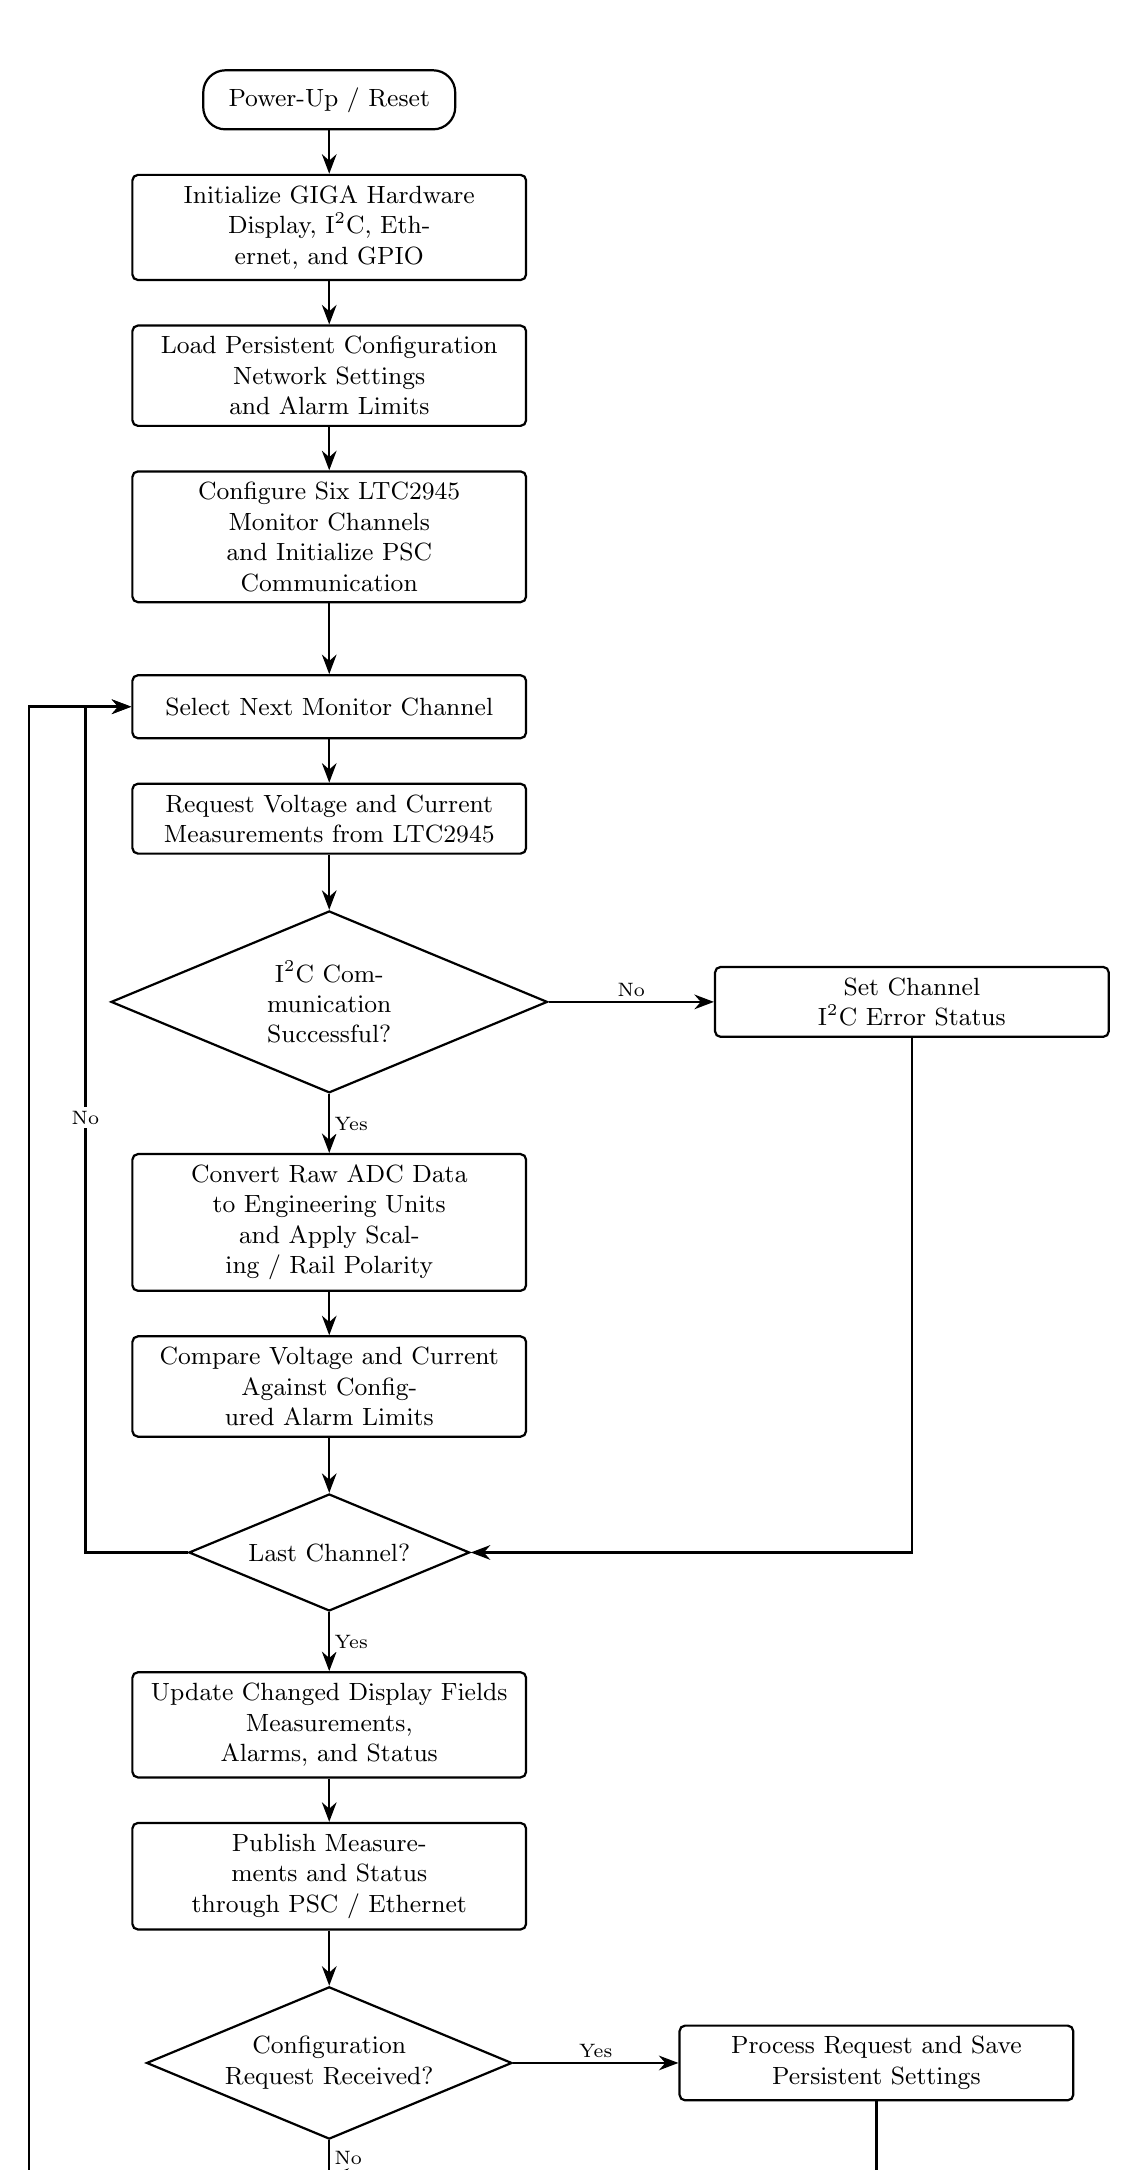
\begin{tikzpicture}[
            >=Stealth,
            font=\small,
            node distance=0.55cm and 1.6cm,
            process/.style={
                draw,
                rectangle,
                rounded corners=2pt,
                align=center,
                minimum width=5.0cm,
                minimum height=0.80cm,
                text width=4.7cm,
                inner sep=4pt,
                line width=0.8pt
            },
            decision/.style={
                draw,
                diamond,
                aspect=2.4,
                align=center,
                text width=2.8cm,
                inner sep=1pt,
                line width=0.8pt
            },
            terminator/.style={
                draw,
                rectangle,
                rounded corners=8pt,
                align=center,
                minimum width=3.2cm,
                minimum height=0.75cm,
                line width=0.8pt
            },
            arrow/.style={
                ->,
                line width=0.9pt
            },
            flowlabel/.style={
                font=\scriptsize,
                fill=white,
                inner sep=1.5pt
            }
            ]

            % ============================================================
            % INITIALIZATION
            % ============================================================

            \node[terminator] (start)
            {Power-Up / Reset};

            \node[process, below=of start] (init)
            {Initialize GIGA Hardware\\
                Display, I\textsuperscript{2}C, Ethernet, and GPIO};

            \node[process, below=of init] (settings)
            {Load Persistent Configuration\\
                Network Settings and Alarm Limits};

            \node[process, below=of settings] (configure)
            {Configure Six LTC2945 Monitor Channels\\
                and Initialize PSC Communication};

            % ============================================================
            % ACQUISITION LOOP
            % ============================================================

            \node[process, below=0.9cm of configure] (select)
            {Select Next Monitor Channel};

            \node[process, below=of select] (read)
            {Request Voltage and Current\\
                Measurements from LTC2945};

            \node[decision, below=0.70cm of read] (comm)
            {I\textsuperscript{2}C Communication\\Successful?};

            % Error branch
            \node[process, right=2.1cm of comm] (error)
            {Set Channel\\
                I\textsuperscript{2}C Error Status};

            % Valid measurement path
            \node[process, below=0.75cm of comm] (convert)
            {Convert Raw ADC Data to Engineering Units\\
                and Apply Scaling / Rail Polarity};

            \node[process, below=of convert] (alarms)
            {Compare Voltage and Current\\
                Against Configured Alarm Limits};

            \node[decision, below=0.70cm of alarms] (last)
            {Last Channel?};

            % ============================================================
            % SYSTEM UPDATE
            % ============================================================

            \node[process, below=0.75cm of last] (display)
            {Update Changed Display Fields\\
                Measurements, Alarms, and Status};

            \node[process, below=of display] (psc)
            {Publish Measurements and Status\\
                through PSC / Ethernet};

            \node[decision, below=0.70cm of psc] (configreq)
            {Configuration\\Request Received?};

            \node[process, right=2.1cm of configreq] (save)
            {Process Request and Save\\
                Persistent Settings};

            % ============================================================
            % PRIMARY FLOW
            % ============================================================

            \draw[arrow] (start) -- (init);
            \draw[arrow] (init) -- (settings);
            \draw[arrow] (settings) -- (configure);
            \draw[arrow] (configure) -- (select);
            \draw[arrow] (select) -- (read);
            \draw[arrow] (read) -- (comm);

            % Communication successful
            \draw[arrow]
            (comm.south)
            --
            node[flowlabel, right] {Yes}
            (convert.north);

            \draw[arrow] (convert) -- (alarms);
            \draw[arrow] (alarms) -- (last);

            % Communication failure
            \draw[arrow]
            (comm.east)
            --
            node[flowlabel, above] {No}
            (error.west);

            % Error skips conversion/alarm processing
            \draw[arrow]
            (error.south)
            |- (last.east);

            % More channels remain
            \draw[arrow]
            (last.west)
            -- ++(-1.3,0)
            |- node[flowlabel, near start, above] {No}
            (select.west);

            % All six channels complete
            \draw[arrow]
            (last.south)
            --
            node[flowlabel, right] {Yes}
            (display.north);

            \draw[arrow] (display) -- (psc);
            \draw[arrow] (psc) -- (configreq);

            % Configuration request
            \draw[arrow]
            (configreq.east)
            --
            node[flowlabel, above] {Yes}
            (save.west);

            % No configuration request:
            % loop back without dropping below the figure
            \coordinate (loopbottom)
            at ($(configreq.south)+(0,-0.45)$);

            \draw[arrow]
            (configreq.south)
            --
            node[flowlabel, right] {No}
            (loopbottom)
            -| ($(select.west)+(-1.3,0)$)
            |- (select.west);

            % After saving configuration, re-enter acquisition loop
            \draw[arrow]
            (save.south)
            |- ($(configreq.south)+(0,-0.45)$);

        \end{tikzpicture}

    \end{adjustbox}

    \caption{
        Top-level Arduino GIGA firmware flowchart. Following initialization,
        the controller continuously acquires measurements from the six LTC2945
        monitoring channels, validates I\textsuperscript{2}C communication,
        converts valid data to engineering units, evaluates configured alarm
        limits, updates the local display, publishes measurements through the
        PSC/Ethernet interface, and services configuration requests.
    }
    \label{fig:firmware-flowchart}

\end{figure}


\subsection{PSC and EPICS Communication Flow}
\label{sec:epics-software-flowchart}
% =====================================================================

The Arduino GIGA does not directly implement EPICS Channel Access. Instead,
measurement and status information is transmitted through the Ethernet
interface using the PSC protocol. The EPICS IOC uses PSCDriver to communicate
with the GIGA, maps the received values into EPICS process variables, and makes
those process variables available to the CS-Studio Phoebus operator interface.

This separation allows the embedded controller to remain responsible for
hardware acquisition and local alarm evaluation while the IOC provides the
interface between the embedded hardware and the facility control system.
Figure~\ref{fig:epics-data-flow} summarizes this software data path.

\begin{figure}[H]
    \centering

    \resizebox{0.95\textwidth}{!}{%
        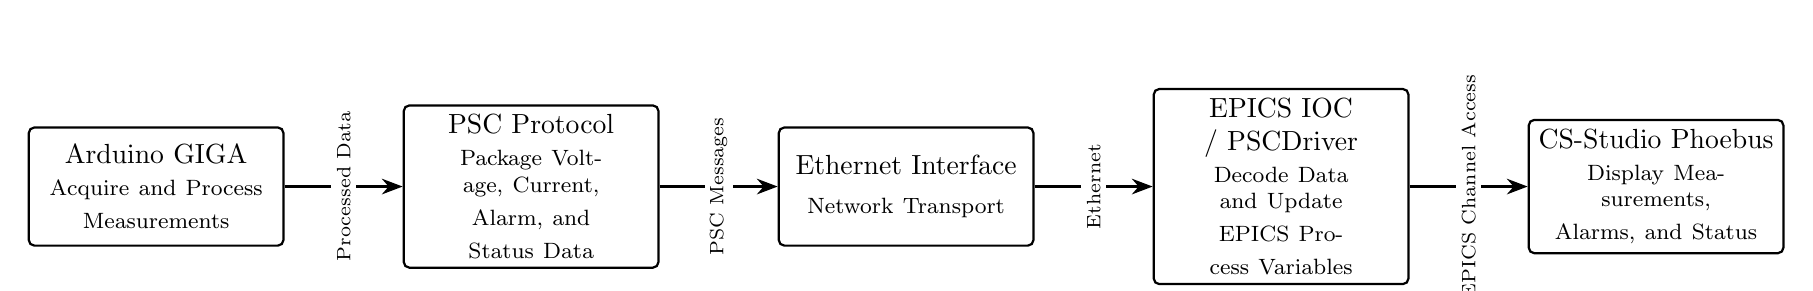
\begin{tikzpicture}[
            >=Stealth,
            node distance=1.25cm,
            process/.style={
                draw,
                rectangle,
                rounded corners=2pt,
                align=center,
                minimum width=3.2cm,
                minimum height=1.5cm,
                text width=3.0cm,
                line width=0.8pt
            },
            arrow/.style={
                ->,
                line width=1.0pt
            },
            siglabel/.style={
                font=\scriptsize,
                fill=white,
                inner sep=2pt,
                rotate=90
            }
            ]

            \node[process] (measure)
            {Arduino GIGA\\[2pt]
                \footnotesize
                Acquire and Process\\
                Measurements};

            \node[process, right=1.5cm of measure] (psc)
            {PSC Protocol\\[2pt]
                \footnotesize
                Package Voltage, Current,\\
                Alarm, and Status Data};

            \node[process, right=1.5cm of psc] (ethernet)
            {Ethernet Interface\\[2pt]
                \footnotesize
                Network Transport};

            \node[process, right=1.5cm of ethernet] (ioc)
            {EPICS IOC / PSCDriver\\[2pt]
                \footnotesize
                Decode Data and Update\\
                EPICS Process Variables};

            \node[process, right=1.5cm of ioc] (phoebus)
            {CS-Studio Phoebus\\[2pt]
                \footnotesize
                Display Measurements,\\
                Alarms, and Status};

            \draw[arrow]
            (measure.east) --
            node[siglabel, midway] {Processed Data}
            (psc.west);

            \draw[arrow]
            (psc.east) --
            node[siglabel, midway] {PSC Messages}
            (ethernet.west);

            \draw[arrow]
            (ethernet.east) --
            node[siglabel, midway] {Ethernet}
            (ioc.west);

            \draw[arrow]
            (ioc.east) --
            node[siglabel, midway] {EPICS Channel Access}
            (phoebus.west);

        \end{tikzpicture}%
    }

    \caption{
        Software communication path from the Arduino GIGA firmware through
        PSCDriver and the EPICS IOC to the CS-Studio Phoebus operator interface.
    }
    \label{fig:epics-data-flow}
\end{figure}


% =====================================================================
\subsection{Software Configuration Management}
\label{sec:software-configuration}
% =====================================================================

Firmware, IOC configuration files, database definitions, and operator-interface
files are maintained under Git version control so that hardware and software
revisions can be associated with a defined project baseline. The current
software implementation and revision history are available in the
\texttt{PS\_Monitor} repository at:

\begin{center}
    \url{https://github.com/capotosto/PS_Monitor}
\end{center}

Changes made during implementation and testing are committed to the repository,
providing traceability between the preliminary design presented in this report
and the final implemented system. The repository therefore serves as the
controlled source for the firmware and control-system software associated with
the project.

\section{Preliminary Component List / Bill of Materials}
\label{sec:bom}

The current bills of materials for the Sensor Board and Arduino Shield Board
are maintained with their respective KiCad hardware-design files in the
project \texttt{hardware} directory. They are included below for reference.

\subsection{Sensor Board Bill of Materials}

\begin{center}
    \includegraphics[
    page=1,
    angle=90,
    width=\textwidth,
    height=0.95\textheight,
    keepaspectratio
    ]{
        ../hardware/Isolated Multi-Rail Power Supply Monitor Sensor Board/%
        Isolated Multi-Rail Power Supply Monitor Sensor Board BOM 8-22-2026 REV -.pdf
    }
\end{center}


\subsection{Arduino Shield Board Bill of Materials}

\begin{center}
    \includegraphics[
    page=1,
    angle=90,
    width=\textwidth,
    height=0.95\textheight,
    keepaspectratio
    ]{
        ../hardware/Isolated Multi-Rail Power Supply Monitor Arduino Shield Board/%
        Isolated Multi-Rail Power Supply Monitor Arduino Shield Board BOM 8-22-2026 REV -.pdf
    }
\end{center}

    % !TeX root = ../main.tex
\chapter{Installing EPICS Base and IOCs}
\label{chap:epics_iocs}

\section{Introduction}
A simple IOC was written to interface the Arduino Giga which monitors the six supplies. The following section details how to install EPICS Base and required modules, and compile the IOC. It is written assuming a Linux environment; this particular build was done on Ubuntu 22.04LTS.

\section{EPICS Installation Overview}
	EPICS installations performed by M. Capotosto loosely follow the below directory structure:

	\begin{itemize}
		\item \texttt{EPICS\_BASE=/epics/base} or \texttt{/epics/base\_[version]} or similar
		\item \texttt{SUPPORT=/epics/support} -- or sometimes MODULES instead of SUPPORT is used.
			\par\bigskip
			\quad Modules required for the PSU monitor are:
			\begin{itemize}[topsep=0pt]
				\item pscdrv: Portable Streaming Controller Driver
			\end{itemize}
		\item \texttt{epics/iocs} - each IOC is cloned into this repository
		\item \texttt{epics/systemd-softioc} - This is a utility for managing IOCs as a system service
	\end{itemize}

\section{Installing EPICS Base and Required Modules}
	\begin{enumerate}
		\item Install Dependencies for Build
			\hspace*{2em} Install git, build-essential, and perl:\\ \texttt{sudo apt -y install git build-essential perl libtirpc-dev re2c libevent-dev autoconf automake libtool pkg-config}
		\item Create the EPICS user group, and the empty EPICS directory: \\
			\hspace*{2em} \texttt{sudo groupadd epics}\\
			\hspace*{2em} \texttt{sudo usermod -aG epics \$USER}\\
			\hspace*{2em} \texttt{newgrp epics}\\
			\hspace*{2em} \texttt{sudo mkdir -p /epics}\\
			\hspace*{2em} \texttt{sudo chown \$USER:epics /epics}\\
			\hspace*{2em} \texttt{sudo chmod 2775 /epics}\\
		\item EPICS Base is cloned into \texttt{/epics/base} via:\\
			\hspace*{2em} \texttt{git clone --recursive -b 7.0} \\ \hspace*{4em}\texttt{https://github.com/epics-base/epics-base.git /epics/base}\\
			\hspace*{2em} \texttt{cd /epics/base}\\
		\item Build EPICS:\\
			\hspace*{2em} \texttt{make clean}\\
			\hspace*{2em} \texttt{make}\\

		\item Create the remaining directory structure:\\
			\hspace*{2em} \texttt{mkdir -p /epics/iocs /epics/modules}\\

		\item Clone PSC Driver:
		\begin{enumerate}
			\item \texttt{cd /epics/modules}
			\item \texttt{git clone https://github.com/mdavidsaver/pscdrv.git pscdrv}
			\item \texttt{cd /epics/modules/pscdrv}
			\item Set up required files in \texttt{configure/RELEASE, configure/RELEASE.LOCAL}
			\item Build with \texttt{make clean}, and \texttt{make}
		\end{enumerate}

		\item Clone Manage IOCs Utility:
		\begin{enumerate}
			\item \texttt{cd /epics}
			\item \texttt{git clone https://github.com/NSLS2/systemd-softioc.git}
			\item Navigate to the repo directory \texttt{cd systemd-softioc}
			\item Make the install script executable and run:\\
			\hspace*{2em}\texttt{sudo chmod +x install.sh}\\
			\hspace*{2em}\texttt{sudo ./install.sh}\\
			\hspace*{2em}\texttt{sudo usermod -aG epics softioc}\\
			\hspace*{2em}\texttt{newgrp}\\
			\hspace*{2em}\texttt{sudo chown softioc:epics /epics/iocs}\\
			\hspace*{2em}\texttt{sudo chmod 2775 /epics/iocs}\\
		\end{enumerate}
	\end{enumerate}

\section{Installing the PSU Monitor IOC}
\begin{enumerate}
	\item Change to IOC directory \texttt{cd /epics/iocs}
	\item Clone the repo:\\
	\hspace*{1em} \texttt{git clone https://github.com/capotosto/PS\_Monitor psuMonitorIOC}
	\item \texttt{cd psuMonitorIOC}
	\item Create the \texttt{RELEASE.local} file, \texttt{touch configure/RELEASE.local}
	\item \texttt{echo -e "EPICS\_BASE = /epics/base\textbackslash n}\\
		\hspace*{2em}\texttt{PSCDRV = /epics/modules/pscdrv\textbackslash n}\\
	\item Build the IOC: \texttt{make clean}, \texttt{make}
	\item Update the st.cmd file as needed: \texttt{cd iocBoot/iocpsuMonitor}
	\item Create the st.cmd file used by systemd-softioc: \begin{verbatim}echo -e '#!/bin/bash\n\n
		cd "/epics/iocs/psuMonitorIOC/iocBoot/iocpsuMonitor"\n./st.cmd' > st.cmd\end{verbatim}
	\item Make the new st.cmd executable: \texttt{chmod +x st.cmd}
	\item Find the next available port: \texttt{manage-iocs nextport}
	\item Configure this in the config file: \texttt{nano config}
	\item Set the \texttt{NAME=}, \texttt{PORT=} your next port, \texttt{USER=softioc}, and \texttt{HOST=\$HOSTNAME}
	\item Update the directory path in the root-level st.cmd to the \texttt{iocBoot/iocpsuMonitor/st.cmd}
	\item Enroll in manage-iocs as a service: \texttt{sudo manage-iocs install psuMonitorIOC}
	\item Enable auto-start on boot: \texttt{sudo manage-iocs enable psuMonitorIOC}
	\item Check the status, it should be running! \texttt{manage-iocs status}
	\item And if you want other information on the ioc: \texttt{manage-iocs report}
\end{enumerate}





















    \include{./TeX_files/CS-Studio-Phoebus}
    % !TeX root = ../main.tex
\chapter{Prototyping and Development}
\label{chap:prototyping-dev}

\section{Introduction}


\section{Testing the LTC2945}
    The LTC2945 testing was carried out using a Linear Tech eval board, DEMO CIRCUIT 1697A. Connections and modifications were made as follows:
    \begin{itemize}
        \item VIN: tied to Arduino +5V
        \item GND: tied to Arduino GND
        \item ADIN: Tied to GND
        \item SCL: Tied to Arduino Pin D8 I2C2 SCL
        \item SDAI/SDAO (JP2 set to TIE): Arduino Pin D9 I2C2 SDA
        \item VPU: Tied to Arduino +3v3
        \item VOUT: Float or tied to dummy load (1k$\Omega$ to 10k$\Omega$)
        \item 20m$\Omega$ shunt replaced with 17$\Omega$ shunt for testing with $\sim$5k$\Omega$ load
        \item Installed 4.7k$\Omega$ pull up on I2C lines via R4, R5 footprints on EVB
    \end{itemize}

    \newpage
    \subsection{Calculating Shunt Value for Test}
    Using the 5V from the arduino as a source, and a load ranging 1k to 10k ohms, we calculate:
    $$R_{L,min}=1k\Omega$$
    $$V_{shunt}=V_S\frac{R_S}{R_L+R_S}$$
    $$R_S=\frac{V_{Shunt}R_L}{V_s-V_{Shunt}}$$
    $$V_{shunt}=0.1024V$$
    $$R_{S,full scale}=\frac{(0.1024V)(1k\Omega)}{5V-0.1024V}=20.91\Omega$$
    Adding some headroom, say, 15\%, and going to an E96 resistor value...
    $$R_S=0.85(20.91)=17.8\Omega$$
    Verifying for the high end of the range:
    $$I_{min}=\frac{5V}{10k\Omega + 17.8\Omega}=499.1\mu A$$
    $$V_{shunt, min}=(499.1\mu A)(17.8\Omega)=8.88mV$$
    The shunt will range from 8.88mV to 87.44mV, within the ADC's usable range of 0V to 102.4mV.

    \newpage
    \subsection{Pictures of Evaluation Board, Display, and Phoebus Panels}
    \begin{figure}[H]
        \centering
        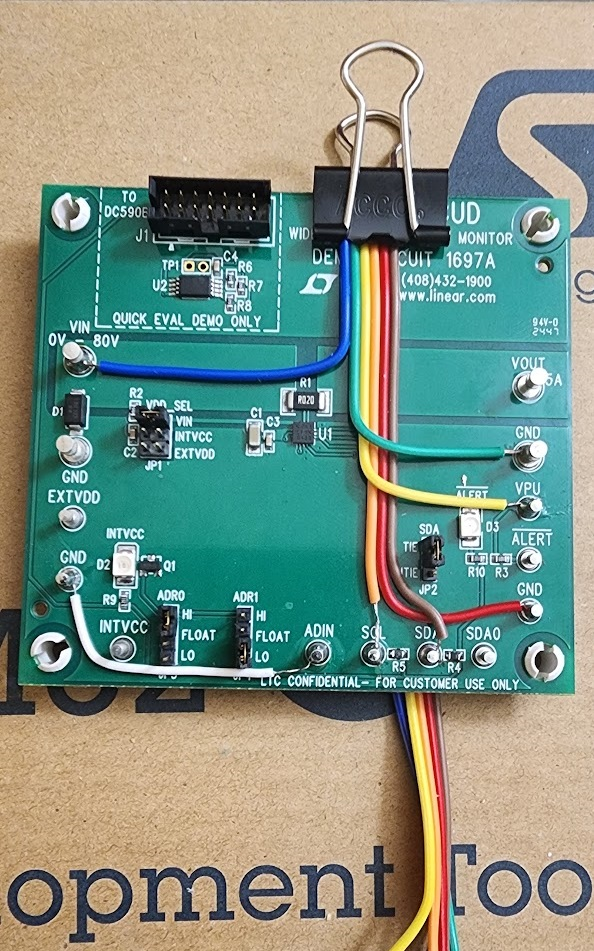
\includegraphics[
        width=3.5in,
        %height=0.85\textwidth,
        keepaspectratio
        ]{Pictures/LTC2945_EVB_Original_Shunt}
        \caption{DEMO CIRCUIT 1697A Eval Board with Original Shunt, fly leads to connect to Arduino.}
    \end{figure}

    \begin{figure}[H]
        \centering
        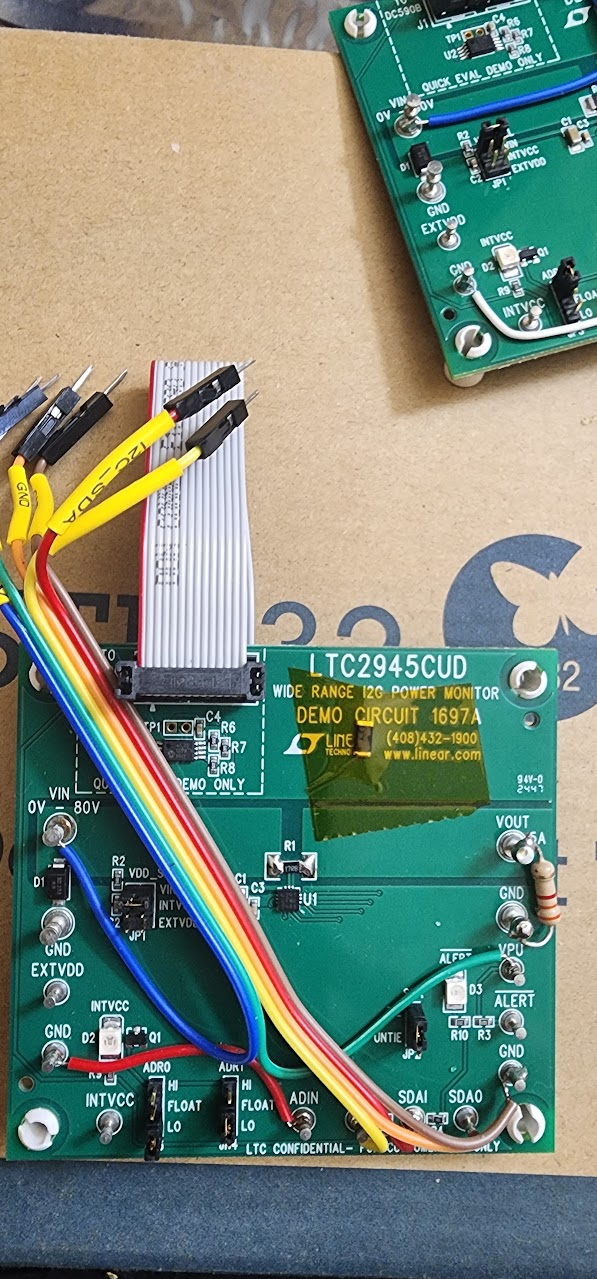
\includegraphics[
        width=3.5in,
        %height=0.85\textwidth,
        keepaspectratio
        ]{Pictures/LTC2945_EVB_17Ohm_Shunt}
        \caption{DEMO CIRCUIT 1697A Eval Board with 17$\Omega$ Shunt, fly leads to connect to Arduino, and 4.7k$\Omega$ test load.}
    \end{figure}

    \begin{figure}[H]
        \centering
        \includegraphics[
        width=3.5in,
        %height=0.85\textwidth,
        keepaspectratio
        ]{Pictures/ExampleDisplay-Single\_EVB_Connected\_Non-ALM}
        \caption{Arduino Giga with GIGA DISPLAY SHIELD showing dummy -5V rail being monitored, without alarm}
    \end{figure}

    \begin{figure}[H]
    \centering
    \includegraphics[
    width=3.5in,
    %height=0.85\textwidth,
    keepaspectratio
    ]{Pictures/ExampleDisplay-Single\_EVB_Connected\_ALM}
    \caption{Arduino Giga with GIGA DISPLAY SHIELD showing dummy -5V rail being monitored, with UVL alarm, other channels I2C ALARM.}
    \end{figure}

    \begin{figure}[H]
        \centering
        \includegraphics[
        width=3.5in,
        %height=0.85\textwidth,
        keepaspectratio
        ]{Pictures/ExampleDisplay-Single\_EVB\_Connected\_Non-ALM-3k3Load}
        \caption{Arduino Giga with GIGA DISPLAY SHIELD showing dummy -5V rail being monitored, without alarm, 3.3k$\Omega$ Load}
    \end{figure}

    \begin{figure}[H]
        \centering
        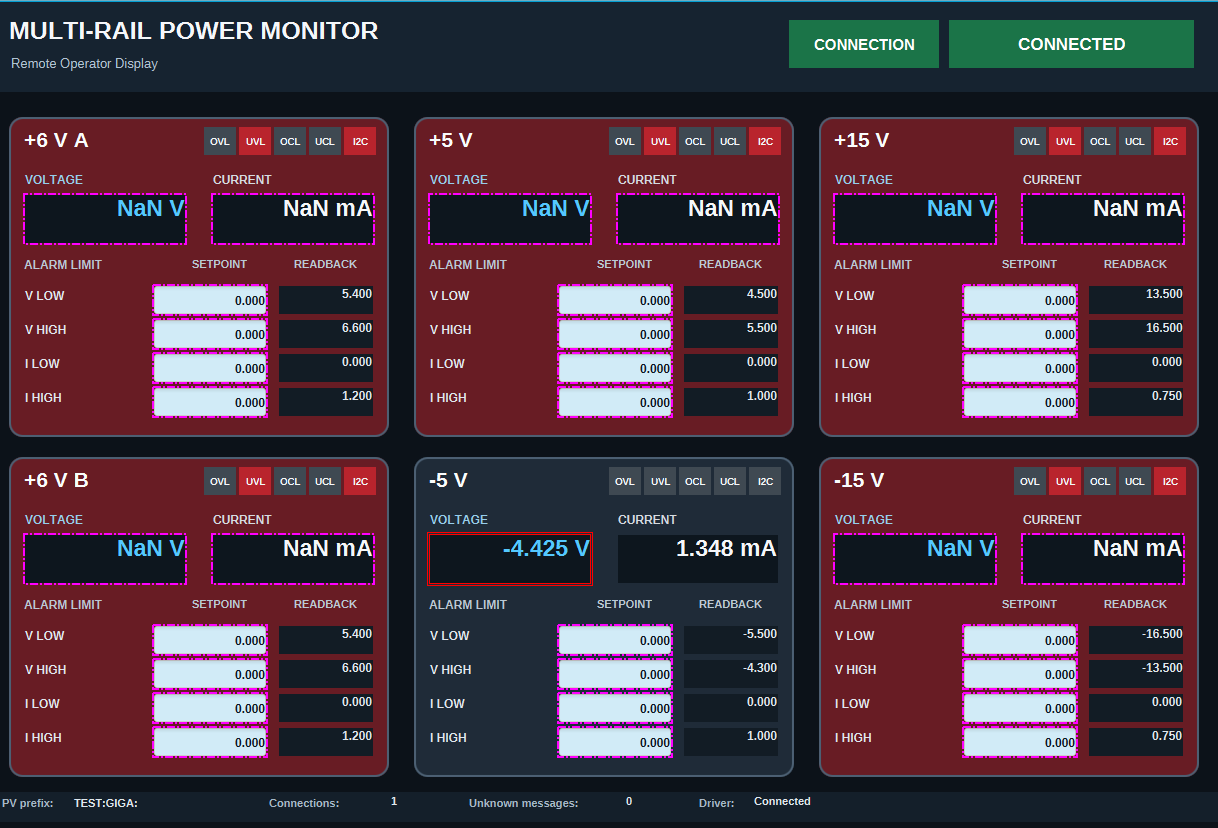
\includegraphics[
        width=\textwidth,
        %height=0.85\textwidth,
        keepaspectratio
        ]{Pictures/Phoebus-SS-N5V-Test-3k3Load}
        \caption{Arduino Giga with GIGA DISPLAY SHIELD showing dummy -5V rail being monitored, without alarm, 3.3k$\Omega$ Load}
    \end{figure}


    \appendix

    \backmatter
    % bibliography, glossary and index would go here.

\end{document}